% ====== GENERIC SECTION TEMPLATE ======
\section{introduction}
\label{sec:introduction} % Label for referencing

The objective of this mini-challenge is to generate high-quality (HQ) face images from corrupted low-quality (LQ) ones. The data for this task is sourced from FFHQ. For this challenge, we have provided a mini dataset comprising of 5000 HQ images for training and 400 LQ-HQ image pairs for validation. Please note that the LQ images are not included in the training set.

As commonly done within SR training, the data is purely synthetic, and constructed "on the fly" by perfomring Gaussian blur, Downsampling, Noise, and Compression on the HQ images to make the LQ images. The LQ images are then used to train the model to generate the HQ images. In figure~\ref{fig:kernels} some of the kernels used to transform the HQ images to LQ images are shown. Note that these are different for each of the samples.


\subsection{Synthetic Data Generation}
\label{subsec:synthetic-data-generation}

\begin{minipage}{\textwidth}
    \centering
    \begin{figure}[H]
        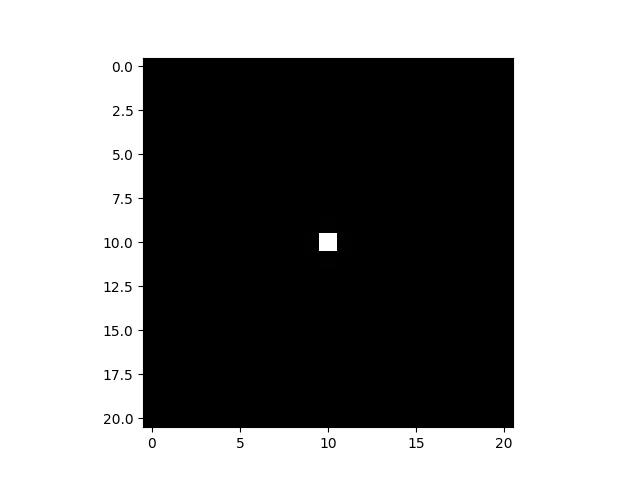
\includegraphics[width=0.3\textwidth]{imgs/kernel1output.png}
        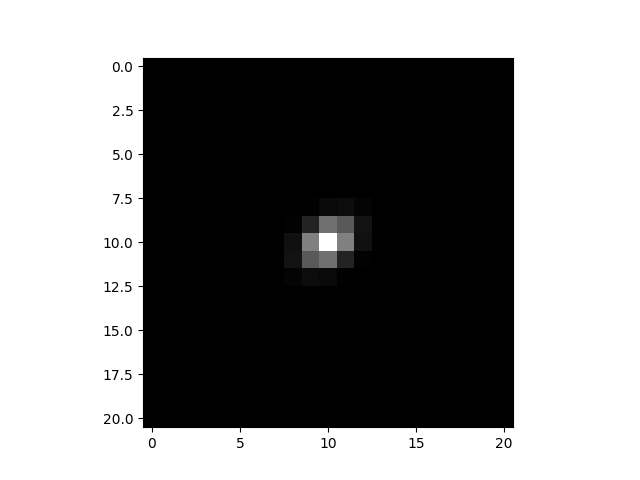
\includegraphics[width=0.3\textwidth]{imgs/kernel2output.png}
        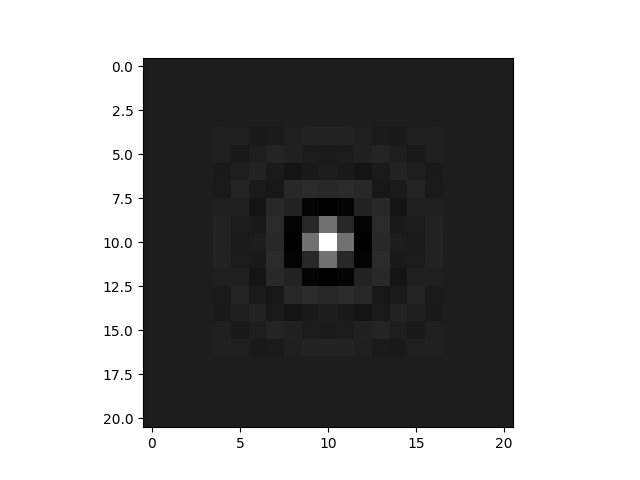
\includegraphics[width=0.3\textwidth]{imgs/sinc_kerneloutput.png}
        \caption{Example kernels in LQ synthesis. Note that each of these kernels is uniquely generated for each low-quality image.}
        \label{fig:kernels}
    \end{figure}
\end{minipage}

This synthetic data generation process follows the methodology described in "Training Real-World Blind Super-Resolution with Pure Synthetic Data" by Wang et al. The process involves the use of various kernels, as illustrated in Figure~\ref{fig:kernels}, to degrade HQ images into LQ images. Each kernel is uniquely generated for each image. The steps in the pipeline include:

\begin{enumerate}
    \item \textbf{Initialization}
    \begin{itemize}
        \item Load configuration options and paths to ground-truth (GT) images.
        \item Initialize the file client based on the configuration.
    \end{itemize}
    
    \item \textbf{Get Item}
    \begin{itemize}
        \item Retrieve and read the GT image for a given index.
        \item Augment the GT image (horizontal flip, rotation).
    \end{itemize}
    
    \item \textbf{Generate Kernels}
    \begin{itemize}
        \item Select kernel size and type (sinc or mixed) based on probability.
        \item Generate and pad the kernel accordingly.
    \end{itemize}
    
    \item \textbf{Apply Final Sinc Filter}
    \begin{itemize}
        \item Optionally apply a final sinc filter.
    \end{itemize}
    
    \item \textbf{Prepare Output}
    \begin{itemize}
        \item Convert and format the image and kernels into tensors.
        \item Return tensors and the image path.
    \end{itemize}
\end{enumerate}

\subsection{Evaluation}
\label{subsec:evaluation} % Label for referencing

The final test set consists of 400 LQ images to evaluate model performance. The evaluation metric is the Peak Signal-to-Noise Ratio (PSNR), a common measure in image processing to assess image quality. Higher PSNR values indicate better image quality, as shown in the following equation:
\begin{equation}
    \text{PSNR} = 10 \cdot \log_{10} \left( \frac{\text{MAX}_I^2}{\text{MSE}} \right)
    \label{eq:psnr}
\end{equation}
